\documentclass[12pt,a4paper]{article}
\usepackage[utf8]{inputenc}
\usepackage[T1]{fontenc}
\usepackage{amsmath}
\usepackage{textcomp}

\usepackage{geometry}
\geometry{a4paper,left=25mm,right=25mm, top=2cm, bottom=2cm} 

\usepackage{graphicx} %fuer bilder

\usepackage{verbatim}




 \usepackage{mathptmx}
 \usepackage[scaled=.90]{helvet}
 \usepackage{courier}



\usepackage{listings}
\usepackage{color}
 
\definecolor{dkgreen}{rgb}{0,0.6,0}
\definecolor{gray}{rgb}{0.5,0.5,0.5}
\definecolor{mauve}{rgb}{0.58,0,0.82}

\pagestyle{empty}
\lstset{numbers=left, language=VHDL}
\lstset{showstringspaces=false,
basicstyle=\ttfamily\footnotesize,
breaklines=true,
tabsize=3,
commentstyle=\color{dkgreen},      % comment style
inputencoding={ansinew},
title=\lstname %zeigt titel der datei an
}

\usepackage{pdfpages} % fuer pdfs
\usepackage{hyperref} % fuer url


%keine einrückungen bei absatz
\parindent 0pt

\begin{document}
\title{Übung 02}
\author{Reinhard Penn, Bernhard Selymes, Robert Zeugswetter}
\date{November 2015}

\normalsize


%Beginn des Dokuments

\newcommand{\Uebung}{ScanChainInsertion}
\newcommand{\srcpath}{../../src}
\newcommand{\simpath}{../../sim}
\newcommand{\synpath}{../../syn}

%Angabe
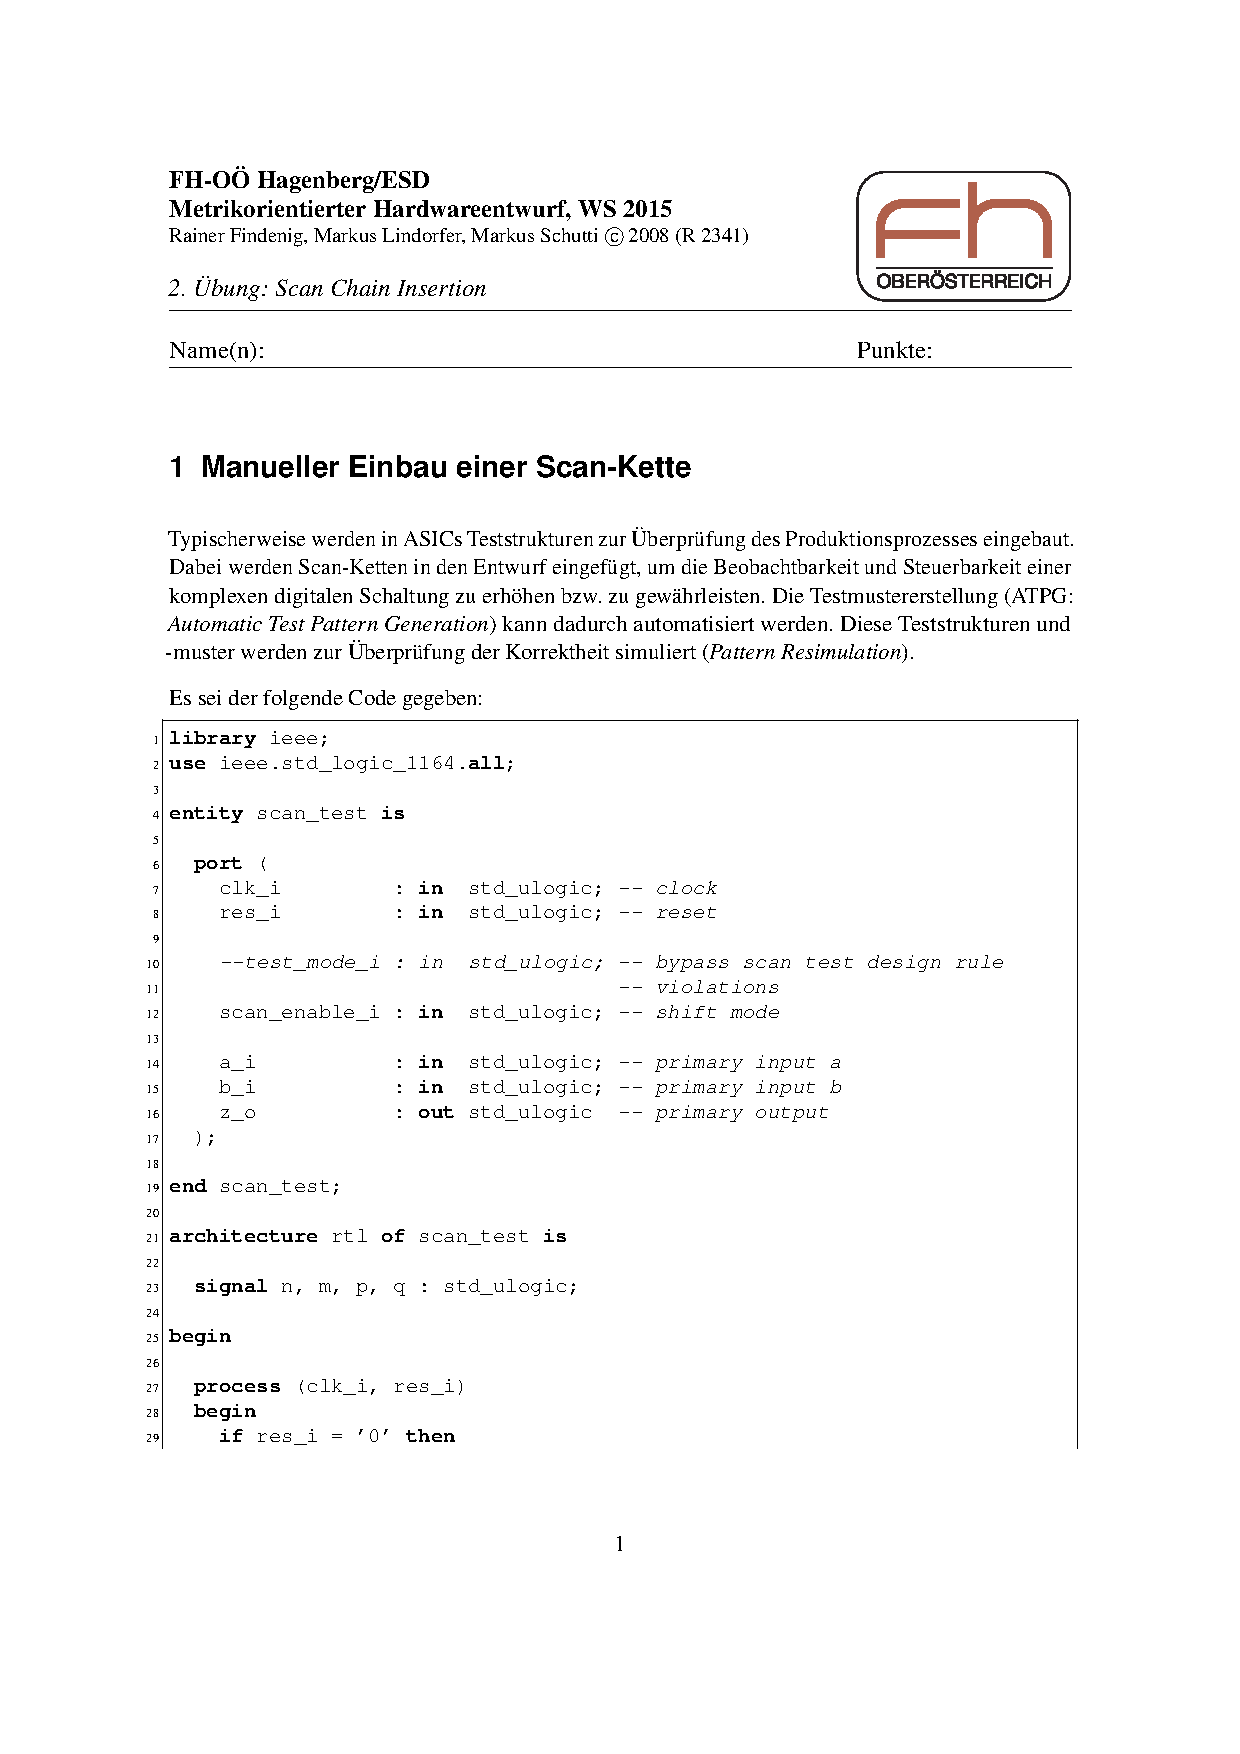
\includepdf[pages=-]{../Angabe.pdf}

\begin{center}
Scan Chain Insertion\\
Übungsprotokoll zur Übung 2\\
Metrikorientierter Hardwareentwurf\\
Bernhard Selymes, Reinhard Penn, Robert Zeugswetter\\
24.11.2015
\end{center}


\section{Manueller Einbau einer Scan-Kette}
Als Flipflops werden DFSC1 und DFSC3 verwendet, da diese die Pendants zu DFC1 und DFC3 sind.\\
Es ist sinnvoll nicht belegte Ausgänge der Flipflops zu verwenden, da sich dadurch die Treiberstärke aufteilt.

\subsection{Erstellen des Testmusters}
\begin{verbatim}
a)
n m p q
1 0 0 0

b)
q = 0
	p = !q
	1 = !0

b_i = 1
	p = ((a_i xor b_i) and b_i) or !(a_i xor b_i)
	
	bei a_i = 0
		((0 xor 1) and 1) or !(0 xor 1) = 1 or !0 = 1
		
	bei a_i = 1
		((1 xor 1) and 1) or !(1 xor 1) = 0 or !0 = 1
\end{verbatim}

\section{Source Code}
\subsection{Manuelle ScanChain}
\lstinputlisting[linerange=32-55, firstnumber=32]{\synpath/netlist/scan_test_mod.vhd}

\subsection{Manuelle ScanChain mit Fehler}
\lstinputlisting[linerange=32-57, firstnumber=32]{\synpath/netlist/scan_test_mod_fail.vhd}

\subsection{Testbench}
\lstinputlisting[linerange=32-57, firstnumber=32]{\srcpath/scan_test_tb.vhd}

\section{Simulation}

\begin{figure}[ht]
\centering
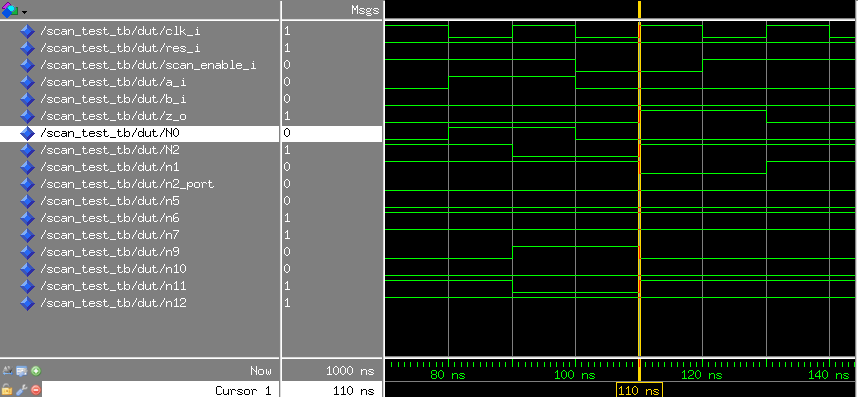
\includegraphics[width=\textwidth]{wave}
\caption{Waveform von Simulation ohne Fehler.}
\end{figure}

\begin{figure}[ht]
\centering
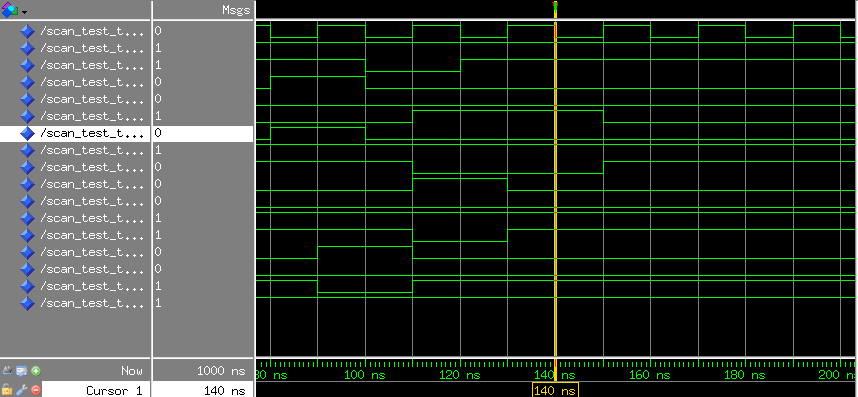
\includegraphics[width=\textwidth]{wave_fail}
\caption{Waveform von Simulation mit Produktionsfehler. Assertion löst aus.}
\end{figure}

\section{DfT-Verletzungen}

\subsection{No asynchronous design style}
Keine asynchronen Elemente (Latch). Diese Latches könnten Daten speichern, was nicht erlaubt ist.
\subsection{No on-chip generation of clock signals}
Für die Flipflops in unserem Design sollte kein selbst erzeugter Takt (das heißt Ausgang eines Flipflops in unserem Design) verwendet werden, da es da beim Umschalten zum Mission Mode zu Fehlern kommen kann.
\subsection{Special attention when more clock domains}
Falls mehrere Clock Domains vorhanden sind muss man spezielle Maßnahmen ergreifen, damit die Scanketten richtig funktionieren. Man könnte zum Beispiel für jede Domain eine eigene Scankette machen.
\subsection{No gating of clock signals}
Clocksignale sollten nicht von anderen Signalen abhängig sein, da ansonsten beim Hineinschieben des Testpattern in die Scankette Probleme auftreten können.
\subsection{No combinatorial feedback loops}
In den kombinatorischen Teilen sollten keine Feedback Loops sein, da es sonst sein kann, dass dort Latches entstehen welche wiederrum Werte speichern können, was nicht erlaubt ist. Wenn die Werte aus der Kombinatorik ins Flipflop geladen werden, dann kann nicht bestimmt werden welchen Wert diese haben.
\subsection{No one-shot delays}
Wenn bei einem Gatter ein Signal an einem Eingang anliegt und bei einem zweiten Eingang das invertierte anliegt, sollte das vermieden werden und stattdessen der negative Q-Ausgang des vorhergehenden Flipsflops verwendet werden.
\subsection{No on-chip generation of asynchronous control signals}
Zum Beispiel die Reset Eingänge der Flipflops sollten nicht durch Kombinatorik in unserer Schaltung erzeugt werden, da dadurch Werte, die beim Schieben durch die Scankette laufen, Flipflops ungewollt resetten könnten.
\subsection{Avoid tristate signals, check for bus contention}
Busses sollten immer auf ein definiertes Potential gezogen werden, da sonst nicht vorhersehbar ist welche Werte sich einstellen, was das Testen unmöglich macht.

\end{document}
